%%%%%%%%%%%%%%%%%%%%%%%%%%%%%%%%%%%%%%%%%
% Journal Article
% LaTeX Template
% Version 1.3 (9/9/13)
%
% This template has been downloaded from:
% http://www.LaTeXTemplates.com
%
% Original author:
% Frits Wenneker (http://www.howtotex.com)
%
% License:
% CC BY-NC-SA 3.0 (http://creativecommons.org/licenses/by-nc-sa/3.0/)
%
%%%%%%%%%%%%%%%%%%%%%%%%%%%%%%%%%%%%%%%%%
%----------------------------------------------------------------------------------------
%       PACKAGES AND OTHER DOCUMENT CONFIGURATIONS
%----------------------------------------------------------------------------------------
\documentclass[fontsize=12pt]{article}
\usepackage{amsmath,amsfonts,amsthm} % Math packages
\usepackage[utf8]{inputenc}
\usepackage[svgnames]{xcolor}
\usepackage[spanish]{babel}
\usepackage{hyperref}
\usepackage{sectsty}
\usepackage{array} 
\usepackage{float}
\usepackage{lipsum} % Package to generate dummy text throughout this template
\usepackage{blindtext}
\usepackage{graphicx} 
\usepackage{xcolor}
\usepackage{caption}
\usepackage{subcaption}
%\usepackage[sc]{mathpazo} % Use the Palatino font
\usepackage[T1]{fontenc} % Use 8-bit encoding that has 256 glyphs
%\linespread{1.05} % Line spacing - Palatino needs more space between lines
\usepackage{sectsty}
\allsectionsfont{\sffamily}
\usepackage{lmodern}
\usepackage[nottoc]{tocbibind}
\usepackage{amsmath}
\usepackage{microtype} % Slightly tweak font spacing for aesthetics
\usepackage[hmarginratio=1:1,top=32mm,columnsep=20pt]{geometry} % Document margins
\usepackage{multicol} % Used for the two-column layout of the document
%\usepackage[hang, small,labelfont=bf,up,textfont=it,up]{caption} % Custom captions under/above floats in tables or figures
\usepackage{booktabs} % Horizontal rules in tables
\usepackage{float} % Required for tables and figures in the multi-column environment - they need to be placed in specific locations with the [H] (e.g. \begin{table}[H])
\usepackage{hyperref} % For hyperlinks in the PDF
\usepackage{lettrine} % The lettrine is the first enlarged letter at the beginning of the text
\usepackage{paralist} % Used for the compactitem environment which makes bullet points with less space between them
\usepackage{abstract} % Allows abstract customization
\renewcommand{\abstractnamefont}{\normalfont\bfseries} % Set the "Abstract" text to bold
\renewcommand{\abstracttextfont}{\normalfont\small\itshape} % Set the abstract itself to small italic text
\usepackage{titlesec} % Allows customization of titles
\usepackage[export]{adjustbox}
\renewcommand\thesection{\arabic{section}} % Roman numerals for the sections
\fontfamily{qag}



\renewcommand{\thesubsection}{\textbf{\textcolor{teal}{\arabic{section}}}\textbf{\textcolor{teal}{.\arabic{subsection}}}}
\renewcommand{\thesubsubsection}{\textbf{\textcolor{teal}{\arabic{section}}}\textbf{\textcolor{teal}{.\arabic{subsection}}}\textbf{\textcolor{teal}{.\arabic{subsubsection}}}}

\titleformat{\section}[block]{\fontsize{18pt}{12pt}\scshape\textcolor{teal}}{\thesection.}{1em}{} % Change the look of the section titles
\titleformat{\subsection}[block]{\fontsize{13pt}{10pt} \textcolor{teal}}{\thesubsection.}{1em}{} % Change the look of the subsection titles
\titleformat{\susubbsection}[block]{\fontsize{10pt}{10pt} \textcolor{teal}}{\thesubsubsection.}{1em}{} % Change the look of the subsubsection titles

\newcommand{\horrule}[1]{\rule{\linewidth}{#1}} % Create horizontal rule command with 1 argument of height
\usepackage{fancyhdr} % Headers and footers
\pagestyle{fancy} % All pages have headers and footers
\fancyhead{} % Blank out the default header
\fancyfoot{} % Blank out the default footer


\lhead[C]{FCEFyN-UNC } % Custom header text
\rhead{
\includegraphics[scale=0.2]{header_unc.jpg}}
\fancyfoot[RO,LE]{\thepage} % Custom footer text
%----------------------------------------------------------------------------------------
%       TITLE SECTION
%----------------------------------------------------------------------------------------
\title{\bigskip \bigskip \bigskip \bigskip \vspace{-15mm}\fontsize{35pt}{35pt}\selectfont\textbf{{Trabajo practico Nº 1: Sockets de internet en sistemas tipo UNIX \\}}
\bigskip \bigskip \fontsize{18pt}{10pt}\selectfont\textbf{\textcolor{teal}{CÁTEDRA DE SISTEMAS OPERATIVOS II}}\bigskip\bigskip \bigskip\bigskip \bigskip}\bigskip\bigskip \bigskip\bigskip \bigskip % Article title
\author{
\large
{
\textsc{Casabella Martin, 39694763 }}\\[2mm]
  martin.casabella@alumnos.unc.edu.ar\\[2mm]
%\thanks{A thank you or further information}\\ % Your name
%\normalsize \href{mailto:marco.torres.810@gmail.com}{marco.torres.810@gmail.com}\\[2mm] % Your email address
\bigskip\bigskip \bigskip \bigskip\bigskip \bigskip
}

\date{\Huge\today}






\usepackage[utf8]{inputenc}

% Default fixed font does not support bold face
\DeclareFixedFont{\ttb}{T1}{txtt}{bx}{n}{8} % for bold
\DeclareFixedFont{\ttm}{T1}{txtt}{m}{n}{8}  % for normal

% Custom colors
\usepackage{color}
\definecolor{deepblue}{rgb}{0,0,0.5}
\definecolor{deepred}{rgb}{0.6,0,0}
\definecolor{deepgreen}{rgb}{4,0.5,0}

\usepackage{listings}

% Python style for highlighting
\newcommand\pythonstyle{\lstset{
language=Python,
basicstyle=\ttm,
otherkeywords={self},             % Add keywords here
keywordstyle=\ttb\color{deepblue},
emph={MyClass,__init__},          % Custom highlighting
emphstyle=\ttb\color{deepred},    % Custom highlighting style
stringstyle=\color{deepgreen},
frame=tb,                         % Any extra options here
showstringspaces=false            % 
}}


% Python environment
\lstnewenvironment{python}[1][]
{
\pythonstyle
\lstset{#1}
}
{}

% Python for external files
\newcommand\pythonexternal[2][]{{
\pythonstyle
\lstinputlisting[#1]{#2}}}

% Python for inline
\newcommand\pythoninline[1]{{\pythonstyle\lstinline!#1!}}

\graphicspath{{Schematics/}}

\sectionfont{\normalsize\sc\leftmark}
%----------------------------------------------------------------------------------------
\begin{document}
\maketitle % Insert title
\thispagestyle{fancy} % All pages have headers and footers

\bigskip
\bigskip
\bigskip
\clearpage

\section{\textbf{Introducción}}
Los sockets son una abstracción de comunicación entre procesos ($IPC$) que en un sistema de tipo UNIX,
se implementan en un descriptor de archivo, sobre el cual se envía o recibe información, al igual que como
se lee o escribe un archivo.\\

Son una herramienta muy importante, uno de los pilares de comunicación entre procesos, y ademas, sumamente utilizada
en la mayoría de las aplicaciones de red.

\section{\textbf{Propósito}}
En este trabajo se pretende entender el funcionamiento de esta abstraccion, donde por un lado se trabaja con la familia de 
sockets UNIX(AF\_UNIX), y por el otro, la familia de sockets TCP/IP (AF\_INET).\\

Se utilizaran para simular la conexión de una estación terrena que se comunica con un 
satélite geostacionario. La estación terrena enviará comandos al satélite y este devolverá
una respuesta y/o realizara cierta acción 


\section{\textbf{Ámbito del sistema}}
Se requiere realizar IPC mediante sockets orientados a conexión y no
orientados a conexión, de ambas familias, UNIX y TCP/IP.\\

Ambos sistemas trabajan con sistemas tipo UNIX. La estación terrena (servidor) estará a la escucha en un
puerto TCP fijo. Antes de levantar la comunicación con el satélite, el usuario debe autenticarse con usuario y contraseña localmente, con
un numero máximo de intentos.Caso contrario, no se provee mecanismo de comunicación ya que el usuario no esta autorizado a interactuar con el satélite.\\
Si el usuario se autentica de forma correcta,el satélite (cliente), deberá poder conectarse al servidor y responder a los comandos ingresados por un prompt desde el
servido.\\



\section{\textbf{Definiciones, Acrónimos y Abreviaturas}}
\subsection{\textbf{\textcolor{blue}{Protocolo TCP}}}
Muchos programas dentro de una red de datos compuesta por redes de
computadoras, pueden usar TCP para crear “conexiones” entre sí a través de las
cuales puede enviarse un flujo de datos. El protocolo garantiza que los datos serán
entregados en su destino sin errores y en el mismo orden en que se transmitieron.
También proporciona un mecanismo para distinguir distintas aplicaciones dentro de
una misma máquina, a través del concepto de puerto.
\subsection{\textbf{\textcolor{blue}{Protocolo UDP}}}
El protocolo de datagramas de usuario es un protocolo del nivel de
transporte basado en el intercambio de datagramas. Permite el envío de
datagramas a través de la red sin que se haya establecido previamente una
conexión, ya que el propio datagrama incorpora suficiente información de
direccionamiento en su cabecera. Tampoco tiene confirmación ni control de flujo,
por lo que los paquetes pueden adelantarse unos a otros; y tampoco se sabe si ha
llegado correctamente, ya que no hay confirmación de entrega o recepción.
\subsection{\textbf{\textcolor{blue}{Dirección IP}}}
La dirección IP es un número que identifica, de manera lógica y jerárquica, a una Interfaz en red (elemento de comunicación/conexión)
 de un dispositivo (computadora, tableta, portátil, smartphone) que utilice el protocolo IP o (Internet Protocol), que corresponde al nivel de red del modelo TCP/IP.
\subsection{\textbf{\textcolor{blue}{Puerto}}}
Un puerto es el valor que se usa, en el modelo de la capa de transporte, para
distinguir entre las múltiples aplicaciones que se pueden conectar al mismo host, o
puesto de trabajo.
\subsection{\textbf{\textcolor{blue}{Sockets IPC}}}
Socket es una forma de IPC (InterProcess Communication) introducida por la Universidad de
Berkeley en su versión de Unix (BSD). El concepto de socket nos evita tener que aprender una
interfaz de programación diferente para cada protocolo.\\
La comunicación por sockets sigue el modelo cliente-servidor
El cliente debe conocer la dirección del servidor para la comunicación, pero el servidor no conoce la existencia del cliente.\\
Una vez establecido el contacto ambas partes pueden enviar y recibir datos, no se reconoce un maestro o esclavo\\
Los procesos generan sockets que son la abstracción utilizada para la comunicación.
A los sockets que van a prestar un servicio se les debe asociar una dirección El cliente utilizando su socket, contacta al servidor (del
que debe conocer la dirección) para transferir datos.
\subsection{\textbf{\textcolor{blue}{Cliente}}}
El cliente es una aplicación informática o un ordenador que consume un
servicio remoto en otro ordenador conocido como servidor, normalmente a través
de una red de telecomunicaciones.
\subsection{\textbf{\textcolor{blue}{Servidor}}}
un servidor basado en software es un programa que ofrece un servicio especial que otros programas denominados clientes pueden usar a nivel local o a través de una red.
La base de la comunicación es el modelo cliente-servidor y, en lo que concierne al intercambio de datos, entran en acción los protocolos de transmisión específicos del servicio.
\subsection{\textbf{\textcolor{blue}{Prompt}}}
Se llama prompt al conjunto de caracteres que se muestran en una línea de
comandos para indicar que está a la espera de órdenes. Éste puede variar
dependiendo del intérprete de comandos.
\clearpage


\section{\textbf{Descripción general del documento}} \label{gral2}
Este documento esta organizado en 6 secciones principales:
\begin{itemize}
\item \label{gra2l}Describe las generalidades del documento y del proyecto
\item \label{dgral} Describe la perspectiva del producto, funciones del mismo, características de usuario y restricciones
\item \label{reqesp} Referencia a los requerimientos del producto, interfaces y casos de uso. Incluye diagramas y gráficos que facilitan su entendimiento
\item \label{diseno} Abarca un diseño de la solución
\item \label{implyresult} La última parte incluye la implementación de la solución y resultados
\item \label{concl} Por último, se encuentran las conclusiones
\end{itemize}


\section{\textbf{Descripción general}} \label{dgral}
\subsection{\textcolor{teal}{\textbf{Perspectiva del Producto}}}
Como objetivo esta el diseño e implementación de un software desarrollado
en lenguaje C basado acatando el modelo cliente/servidor, permitiendo
la comunicacion entre ambas partes a través de sockets de internet y tipo UNIX.\\
El servidor proveerá al usuario un medio para ejecutar acciones definidas y obtener información del cliente remoto a través de un prompt.
\subsection{\textcolor{teal}{\textbf{Funciones del Producto}}}
\subsubsection{\textcolor{orange}{\textbf{Conexión}}}
Permite establecer una conexión mediante socket TCP, desde el cliente al
servidor en la estación terrena. A su vez, puede emplearse el mismo software pero utilizando
la familia de sockets UNIX.
\subsubsection{\textcolor{orange}{\textbf{Autenticación}}}
Característica del servidor, que verificará la existencia de login
(usuario, password) y dará o no autorización al shell interactivo. De haber sido autenticado correctamente,
se levanta la comunicacion con el satélite.
\subsubsection{\textcolor{orange}{\textbf{Prompt interactivo}}}
Luego de una autenticación el servidor esta a la espera de clientes, cuando
estos se conectan provera el prompt al usuario.
\subsubsection{\textcolor{orange}{\textbf{Telemetría}}}
El cliente obtiene y envia ciertos datos de telemetría definidos y los envía al servidor.
\subsubsection{\textcolor{orange}{\textbf{Update firmware}}}
El servidor puede enviar un nuevo firmware destinado a ser cargado en el cliente, que se reiniciara levantando el nuevo archivo binario (firmware).
\subsubsection{\textcolor{orange}{\textbf{Start scanning}}}
El satélite puede iniciar el escaneo de la cara de la tierra y enviarla al servidor en formato de archivo.

\subsection{\textcolor{teal}{\textbf{Características de los Usuarios}}}

\begin{table}[H]
\centering
\begin{tabular}{ |c|c|c| }
 \hline
  \multicolumn{3}{|c|}{\textbf{Autenticacion}}\\
  \hline 
\textbf{Funcion}&\textbf{Cliente} & \textbf{Servidor}\\
 \hline
 Solicitar usuario &&x\\
 Solicitar contrasena &&x\\
 Validar ingreso en la base de datos &&x\\
 Enviar mensaje en funcion al resultado &&x\\
 Levantar socket en caso de loggeo exitoso&&x\\
 No permitir la conexion en caso fallido&&\\
  \hline
\end{tabular}
\bigskip \bigskip \bigskip 
\end{table}


\begin{table}[H]
\centering
\begin{tabular}{ |c|c|c| }
 \hline
  \multicolumn{3}{|c|}{\textbf{Prompt interactivo}}\\
  \hline 
\textbf{Funcion}&\textbf{Cliente} & \textbf{Servidor}\\
 \hline 
 Solicitar prompt &&x\\
 Autenticar usuario &&x\\
 Levantar socket TCP&&x\\
 Codificación y envío de comandos&x&x\\
 Ejecución de comandos localmente&x&\\
 envío y recepción de datos full duplex&x&x\\
  \hline
\end{tabular}
\bigskip \bigskip \bigskip
\end{table}


\begin{table}[H]
\centering
\begin{tabular}{ |c|c|c| }
 \hline
  \multicolumn{3}{|c|}{\textbf{Update firmware}}\\
  \hline 
\textbf{Función}&\textbf{Cliente} & \textbf{Servidor}\\
 \hline 
Ingreso comando firmware update &&x\\
 Validación comando firmware update &&x\\
 Envio de archivo binario &&x\\
 Chequeo de existencia del archivo &&x\\
 Informe de errores emergentes (de haber) &&x\\
 Recibir archivo binario (firmware) y lanzarlo &x&\\
  \hline
\end{tabular}
\bigskip \bigskip \bigskip
\end{table}

\begin{table}[H]
\centering
\begin{tabular}{ |c|c|c| }
 \hline
  \multicolumn{3}{|c|}{\textbf{Start scanning}}\\
  \hline 
\textbf{Función}&\textbf{Cliente} & \textbf{Servidor}\\
 \hline 
Ingreso comando start scanning &&x\\
 Validación comando  start scanning &&x\\
Obtención del archivo(escaneo) &x&\\
 Informe de errores emergentes (de haber) &x&\\
 Envio de archivo jpg &x&\\
 Recepcion y almacenamiento del archivo &&x\\
  \hline
\end{tabular}
\bigskip \bigskip \bigskip
\end{table}


\begin{table}[H]
\centering
\begin{tabular}{ |c|c|c| }
 \hline
  \multicolumn{3}{|c|}{\textbf{Telemetria}}\\
  \hline 
\textbf{Función}&\textbf{Cliente} & \textbf{Servidor}\\
 \hline 
Ingreso comando get telemetry &&x\\
Levantar socket UDP a la espera de resultado de ejecución &&x\\
Levantar socket UDP para comunicación y envio &x&\\
Recolección de datos &x&\\
Envío de datos mediante socket UDP &x&\\
Interpretación y muestra de resultado de ejecución&&x\\
  \hline
\end{tabular}
\bigskip \bigskip \bigskip
\end{table}






\subsection{\textcolor{teal}{\textbf{Restricciones}}}
Las aplicaciones deben compilarse y ejecutarse en sistemas operativos UNIX con permisos para levantar sockets y nuevos procesos.\\
Si se utiliza el software con la familia de sockets UNIX, al ingresar el comando \textbf{update firmware}, se deberá volver a correr el programa.\\
Deben respetarse los nombres de los directorios, y de no existir, se deben crear en sus respectivos path previo a compilar y ejecutar el programa.\\
\subsection{\textcolor{teal}{\textbf{Suposiciones y Dependencias}}}
Ambos sistemas deben representar de la misma forma los número Little Endian o Big Endian.\\
Ambos host deben ser directamente alcanzables por ethernet.\\
Para la compilación es totalmente necesario tener instalados las librerías $GNU$ $GlibC >= 2.2$, para la estandarización de tipos.
\section{\textbf{Requisitos específicos}} \label{reqesp}
Se detallan a continuación los requisitos específicos del sistema, especificados por
el cliente.\\
\subsection{\textcolor{teal}{\textbf{Interfaces externas}}}
En esta sección se especifican los requisitos del proceso de desarrollo de software, como la interfaz de la aplicación, la hardware y entorno del sistema.
La interfaz de usuario del cliente y del servidor serán por cualquier TTY, como por ejemplo una consola interactiva como bash o xterm,.
Para el desarrollo del software se utiliza utiliza GNU/Linux, herramientas de compilación y librerías en su última versión estable, específicamente las versiones
que cumplen los criterios son las rolling release como ArchLinux, Antergos, Manjaro y derivados.
\begin{itemize}
\item Kernel >= 5.0.7 ( 5.0.7-1-ARCH aarch64 GNU/Linux)
\item GCC >= version 8.2 (Provee mejor soporte gnu11/c11)
\item GLibC >= 2.26 (Provee soporte de unificación/comunicacion de tipos para diferentes arquitecturas)
\item Make >= 4.2.1
\item libnet >= 1.1.6-3
\end{itemize}

\subsection{\textcolor{teal}{\textbf{Requisitos funcionales}}}
\subsubsection{\textbf{Requisitos de conexión}}
\begin{enumerate}
\item Debe poder establecerse una conexión libre de errores entre los clientes y el servidor para la transferencia de información.
\item En caso de imposibilidad de conexión debe ser notificado
\item El servidor debe poder ingresar ingresa usuario y contraseña para solicitar acceso alsistema
\item Luego de autentificar se levanta el servidor
\item No se aceptan ni envían comandos previo a autenticar al usuario.
\item El cliente debe ser capaz de detectar una caída de conexion o un rechazo de la misma por errores de la red o por fallo en la autentificación.
\end{enumerate}


\subsubsection{\textbf{Requisitos de conexión}}
\begin{enumerate}
\item Debe poder establecerse una conexión libre de errores entre los clientes y el servidor para la transferencia de información.
\item En caso de imposibilidad de conexión debe ser notificado
\item El servidor debe poder ingresar ingresa usuario y contraseña para solicitar acceso alsistema
\item Luego de autentificar se levanta el servidor
\item No se aceptan ni envían comandos previo a autenticar al usuario.
\item El cliente debe ser capaz de detectar una caída de conexion o un rechazo de la misma por errores de la red o por fallo en la autentificación.
\end{enumerate}

\subsubsection{\textbf{Requisitos de prompt}}
\begin{enumerate}
\item No es posible ingresar comandos si no hay clientes conectados
\item El servidor provee prompt solo si se autenticar correctamente
\item Los comandos se ingresan solo si termino la ejecución del comando anterior, ya sea correctamente o si surgió algún error.
\item Debe identificar si el comando no existe
\item Debe salir del prompt si pierde conectividad con el cliente
\end{enumerate}

\subsubsection{\textbf{Requisitos autenticacion}}
\begin{enumerate}
\item El servidor debe poder verificar al usuario que intenta solicitar un prompt en una base de datos
\item Los usuarios o contraseñas no superaran los 20 caracteres
\item La base de datos debe estar guardada en un archivo de texto plano
\item En caso de fallo de autentificación 3 veces seguidas el servidor debe terminar la aplicación
\item No se aceptan ni envían comandos previo a autenticar al usuario.
\item El cliente debe ser capaz de detectar una caída de conexion o un rechazo de la misma por errores de la red o por fallo en la autentificación.
\end{enumerate}


\subsubsection{\textbf{Requisitos de Update Firmware}}
\begin{enumerate}
\item El único comando aceptado para esta función es ''update firmware''
\item El archivo a enviar es el firmware por TCP
\item El archivo a enviar debe situarse en el directorio cuyo nombre es firmware dentro del directorio del servidor. 
\item El archivo binario puede reemplazarse respetando formato 
\item  El cliente debe recibir el archivo, guardarlo cerrarse y lanzar su nueva actualización por el archivo recibido
\end{enumerate}

\subsubsection{\textbf{Requisitos de Start Scanning}}
\begin{enumerate}
\item El único comando aceptado para esta función es “start scanning”
\item En el escaneo enviar el archivo con el nombre "aerial\_earth\_image\.jpg”
\item El archivo se transmite por TCP
\item El archivo debe situarse en el directorio nombrado img dentro del directorio server
\item El archivo jpg puede reemplazarse respetando formato 
\end{enumerate}


\subsubsection{\textbf{Requisitos de telemetría}}
\begin{enumerate}
\item El único comando aceptado para esta función es “get telemetry”
\item El comando se envia por TCP pero su respuesta es por UDP
\item El servidor debe levantar el socket para escuchar al cliente
\item El comando debe enviar informacion de: ID satelite, uptime, version del firmware, uso RAM
\end{enumerate}


\subsubsection{\textbf{Requisitos de shutdown}}
\begin{enumerate}
\item El único comando aceptado para esta función es “ shutdown now”
\item El comando se envia por TCP 
\item El servidor debe cerrar su socket y el programa debe finalizar
\item El cliente debe cerrar su socket y el programa debe finalizar
\item El usuario recibe un mensaje a traves del prompt que finalizo el programa y ya no puede interactuar con el prompt
\end{enumerate}

\subsection{\textcolor{teal}{\textbf{Requisitos de rendimiento}}}
El sistema debe ser capaz de correr en un SoC (System On Chip) o una computadora personal
(x86/AMD64), con al menos 1[GB] de RAM y 1[GB] de espacio libre, un procesador con
una frecuencia de 1[GHz] contando que solo compite en los recursos con los
procesos del sistema operativo base.
El sistema operativo base puede ser GNU/Linux o derivados de BSD.
\subsection{\textcolor{teal}{\textbf{Restricciones de diseño}}}
No se utilizaron restricciones de diseño en el desarrollo del sistema.
\subsection{\textcolor{teal}{\textbf{Atributos del Sistema}}}
El atributo más importante del sistema es la portabilidad, la capacidad de la
utilización de sistemas operativos tipo UNIX y los escasos recursos necesarios
para correr el software lo hacen ideal para pequeños sistemas embebidos de bajos
recursos
\section{\textbf{Diseño de la solución}} \label{diseno}
La solución está documentada en el repositorio del proyecto.
\href{https://github.com/martincasabella/OSII_2019}{[Repositorio del Proyecto]}

\section{\textbf{Implementacion y resultados}} \label{implyresult}

\begin{figure}[H]
\centering
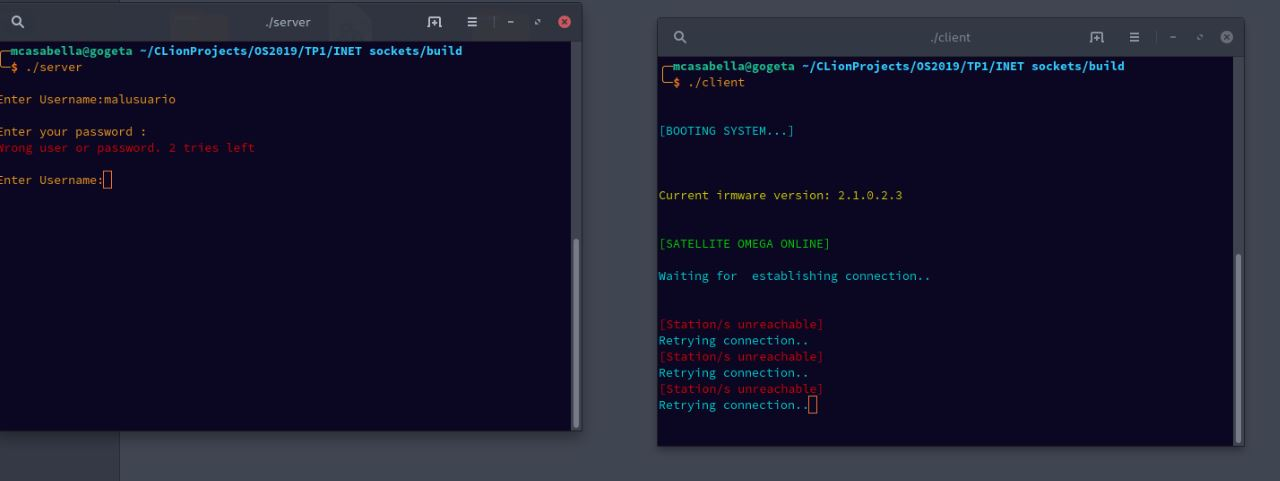
\includegraphics[scale =0.48]{wrong_user.jpg}
\caption{Mal ingreso de usuario}
\bigskip \bigskip \bigskip 
\end{figure}

\begin{figure}[H]
\centering
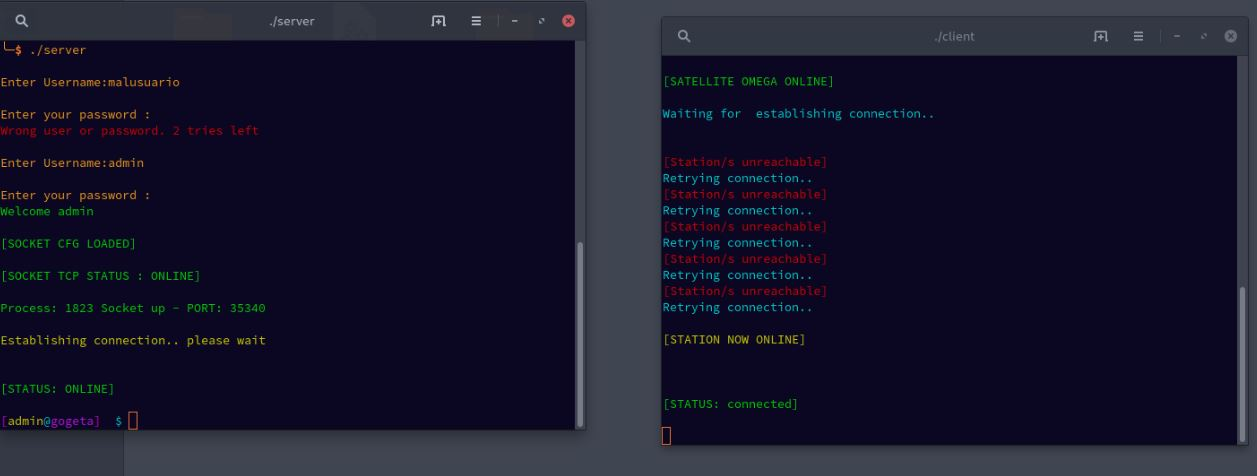
\includegraphics[scale =0.52]{correct_user.jpg}
\caption{Ingreso correcto de usuario}
\bigskip \bigskip \bigskip \bigskip \bigskip \bigskip \bigskip 
\end{figure}

\begin{figure}[H]
\centering
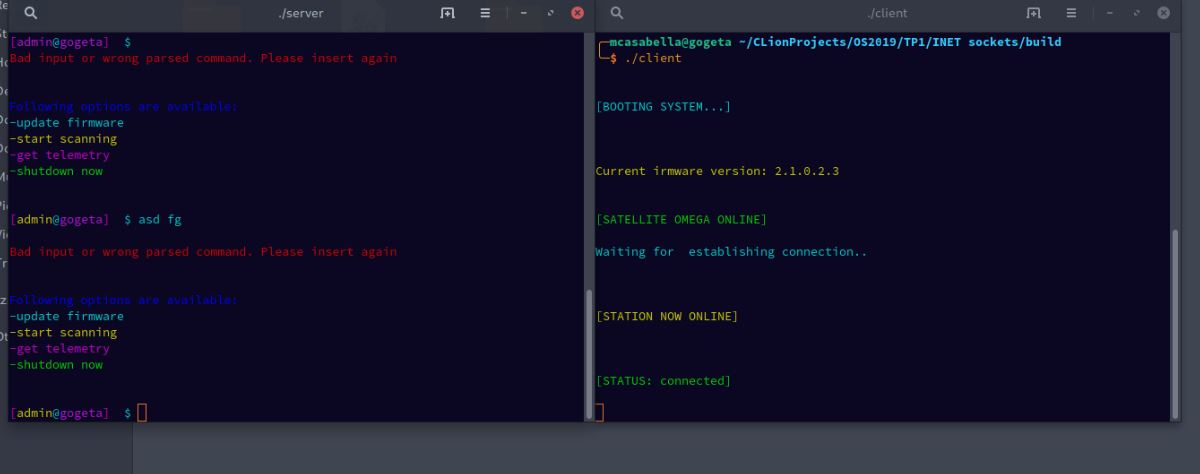
\includegraphics[scale =0.52]{bad_command.jpg}
\caption{Ingreso de comando erroneo}
\end{figure}


Se cita la siguiente secuencia de comandos: primero se ingresa \textbf{get telemetry}, para obtener información del satelite. Se resalta ahi la versión del firmware actual:\\
\begin{figure}[H]
\centering
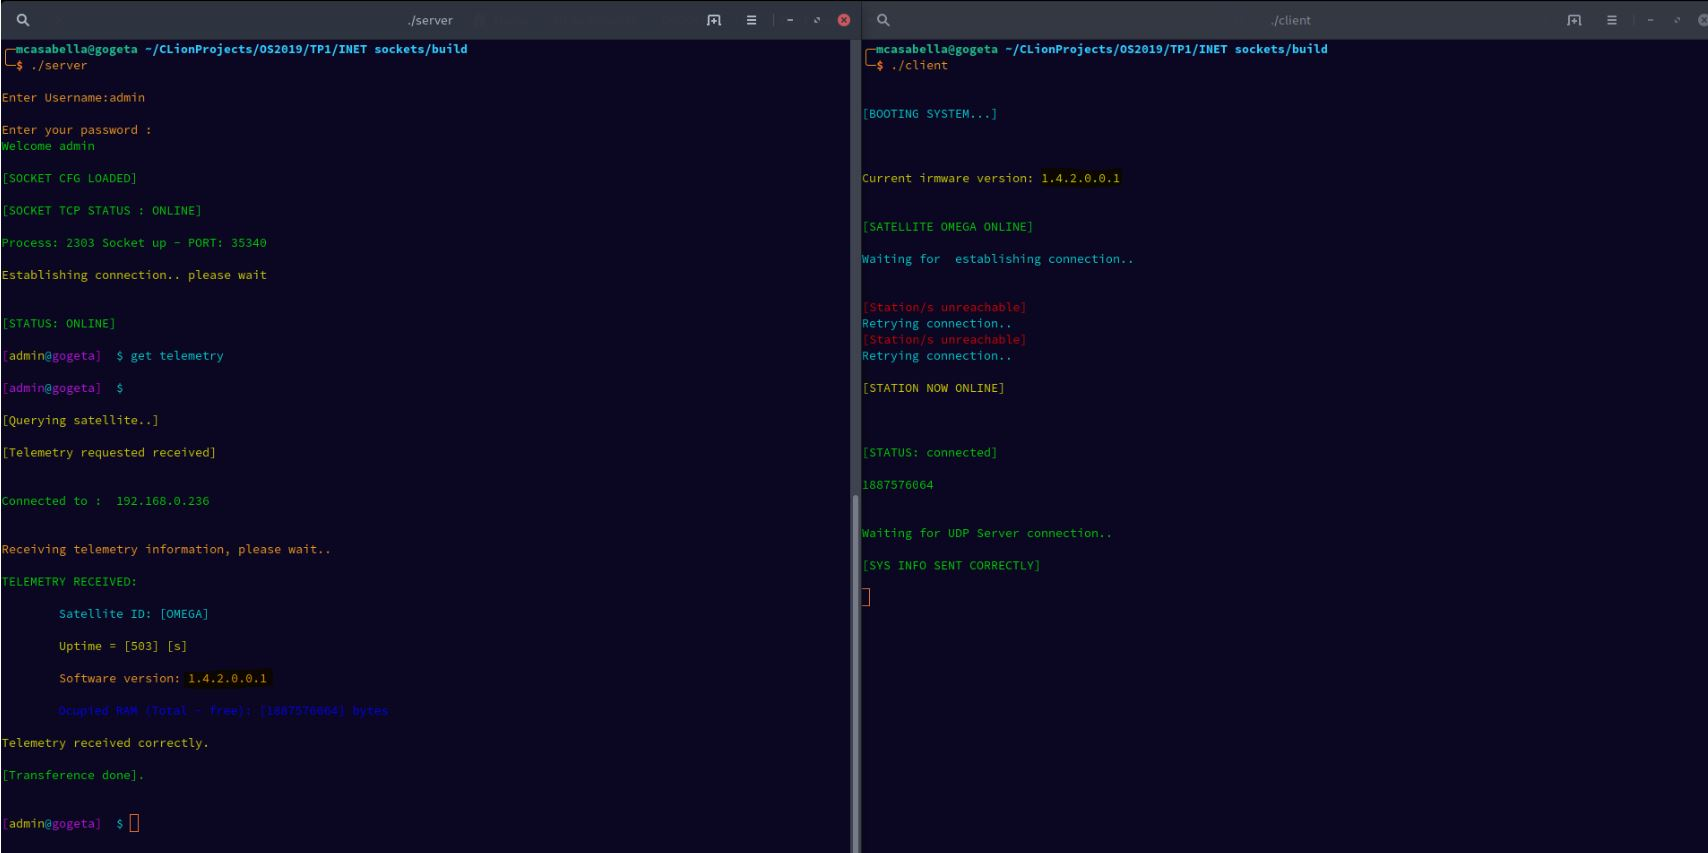
\includegraphics[scale =0.36]{get_tel.jpg}
\caption{Resultado de get telemetry}
\end{figure}

\clearpage
Ahora se ingresa \textbf{update firmware}, para forzar al satélite a actualizarse:\\

\begin{figure}[H]
\centering
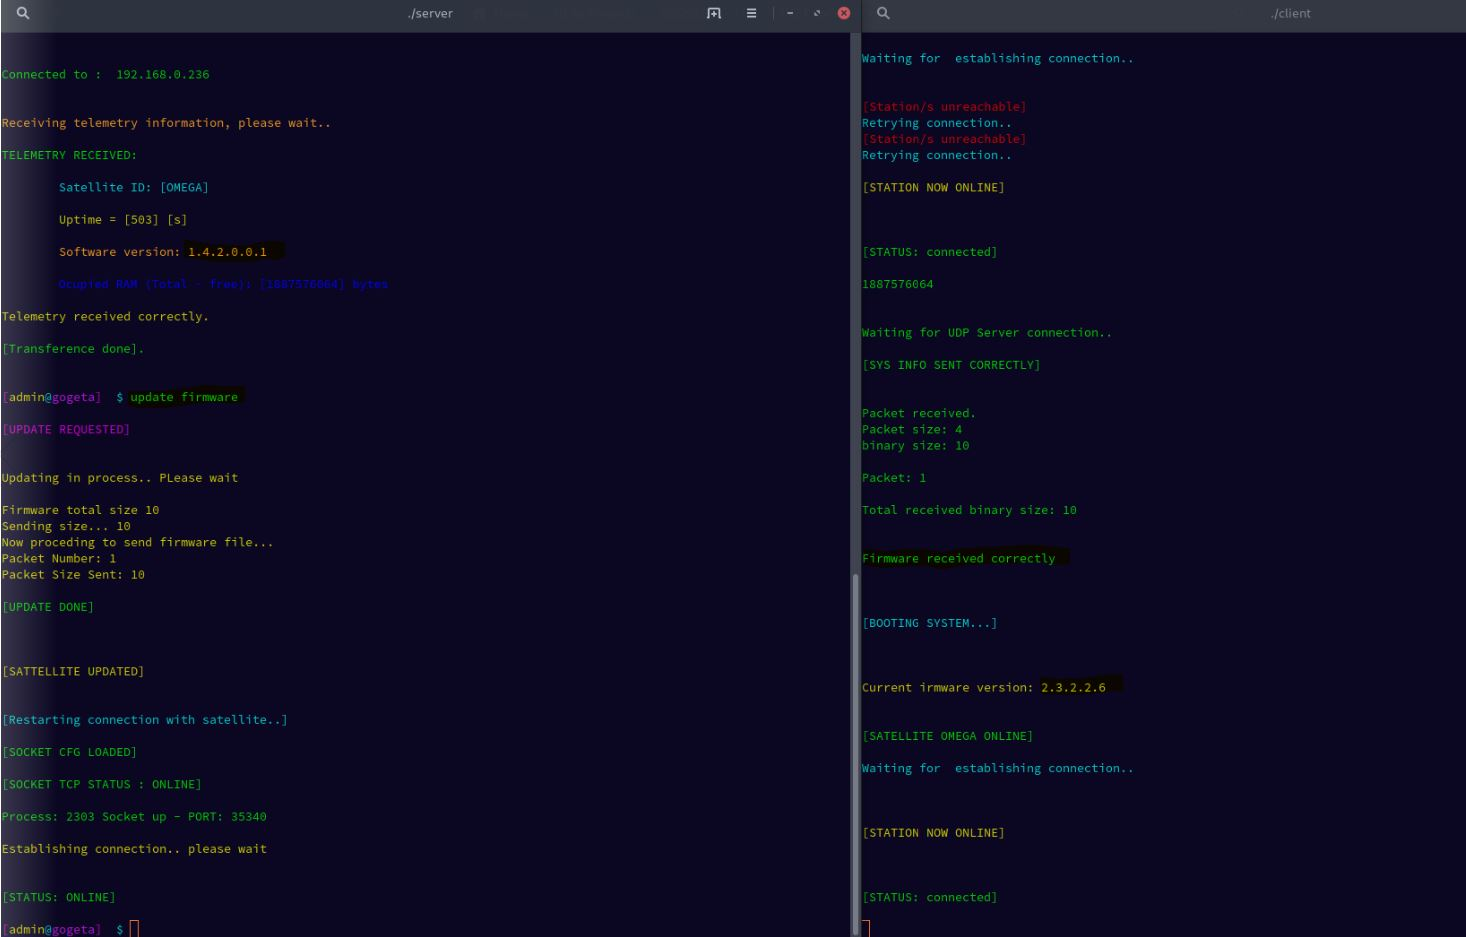
\includegraphics[scale =0.42]{new_firmw.jpg}
\caption{Actualización de firmware}
\end{figure}

Y finalmente, se vuelve a ingresar \textbf{get telemetry} para corroborar si el satélite se actualizo: \\

\begin{figure}[H]
\centering
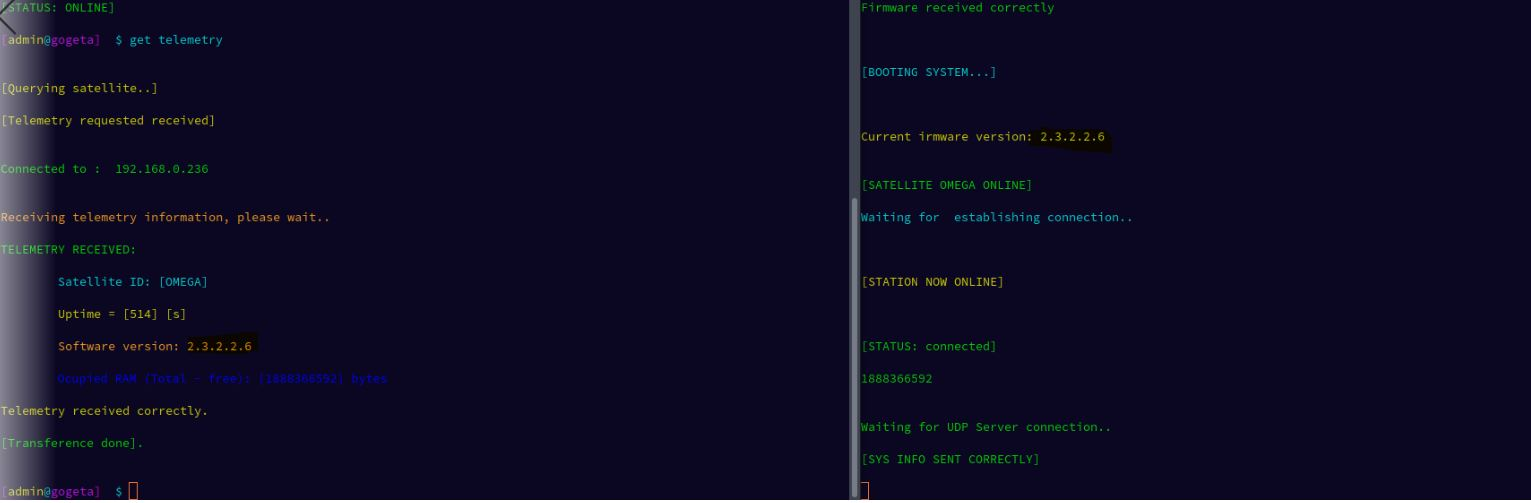
\includegraphics[scale =0.37]{get_new_firmw.jpg}
\caption{Resultado luego de actualizar el satélite}
\end{figure}

Se anexan los restantes comandos:\\

\begin{figure}[H]
\centering
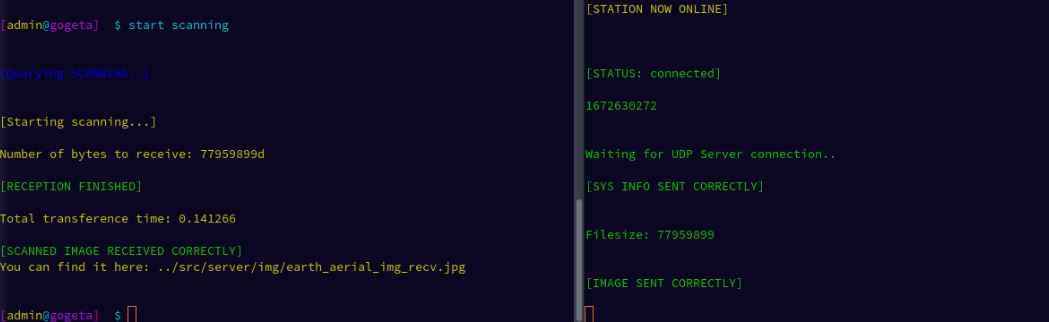
\includegraphics[scale =0.60]{start_scanning.jpg}
\caption{Resultado de start scanning}
\end{figure}



\begin{figure}[H]
\centering
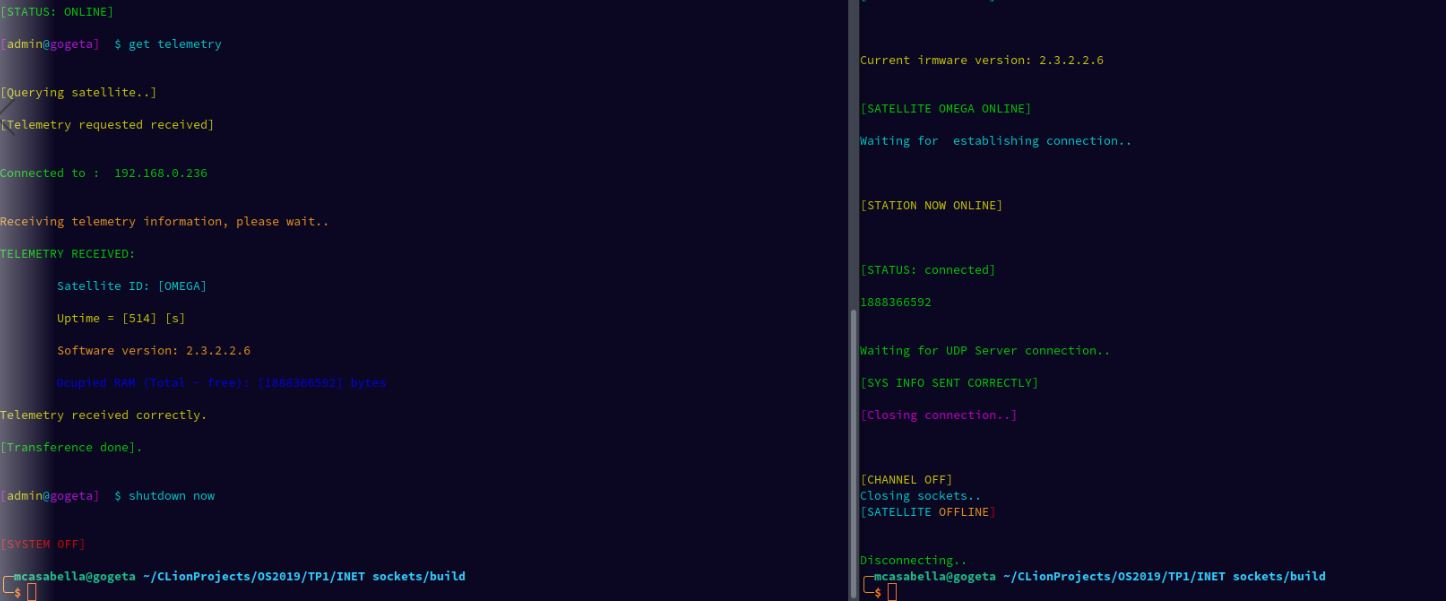
\includegraphics[scale =0.45]{shutdown_now.jpg}
\caption{Apagado de sistema}
\end{figure}



\section{\textbf{Conclusiones}}\label{concl}
Se puso en práctica una forma de IPC, tanto para comunicación de procesos por Internet, a nivel local.
Se maduraron conceptos relacionados al protocolo, las formas de comunicación (bloqueante, o no bloqueante)
y se incorporo la transferencia de información con los mecanismos de abstracción mencionados.\\
\clearpage

\nocite{*}
\bibliography{biblio}

\end{document}


%----------------------------------------------------------------------------------------
%\end{multicols}
\end{document}




